In the last section of this chapter the result of the simulation of the Sr-90 source as described up to this point is presented. The purpose is to study the dose deposition in the PTW chamber TM33053 when it is irradiated by a $\beta^-$ source. In this simulation, the chamber has the same corrosion layer as the simulations presented in Chapter 3. 

\clearpage
The tally +F6 is:

\begin{figure}[!h]
    \centering
    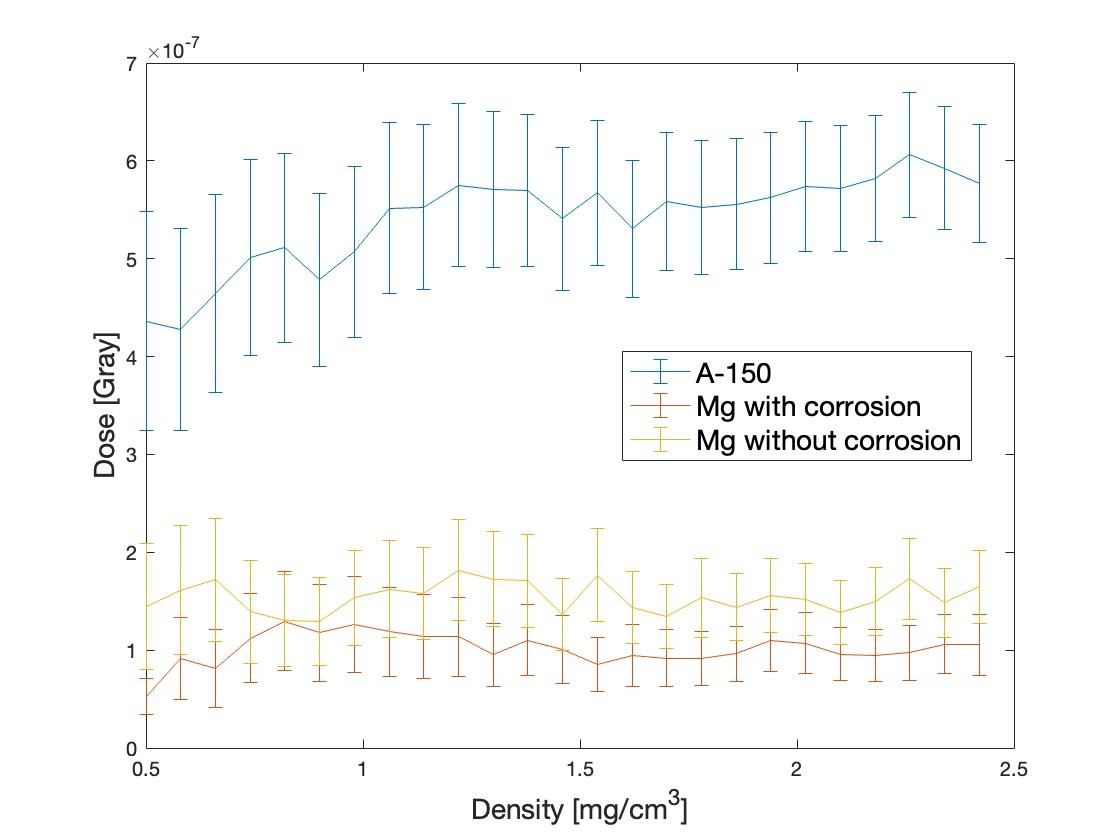
\includegraphics[scale = 0.32]{Master Thesis Manuel Galdon/figures/check source/+f6.jpg}
    \caption{Simulation of PTW-33053 with a 0.37 \unit{\milli\meter} thick layer of hydromagnesite on all magnesium surfaces using the check source, without a corrosion layer, and TE chamber. The magnesium chamber has been simulated without a concentration of water. Tally +F6.}
  \label{fig:PTW-33053 with hydromagnesite. Tally +F6. Electrons}
\end{figure}

It is shown in Figure \ref{fig:PTW-33053 with hydromagnesite. Tally +F6. Electrons} that the dose deposition in the magnesium chamber is constant along the density of argon and almost the same for the simulation with and without the corrosion layer. This is the expected response. %because the electrons are principally scattered by the magnesium and do not trigger a nuclear reaction. Therefore, the dose shown in the plot is basically delivered by secondary particles.

The result of the TM33053 chamber is also expected. The dose in the TE chamber is although of the same order of magnitude, higher than the magnesium chamber. This outcome is due to the higher sensibility of this chamber, as it has been confirmed in the PTB calibration. On the other hand, it is due to the higher complexity of the composition of the A-150 tissue equivalent plastic in comparison with magnesium. %This complexity leads to a higher number of interactions and therefore to the generation of further secondary particles.

%The dose delivered by the secondary particles has been tallied in this problem and it has not been shown in this work. The reason for it is, either the dose is several orders of magnitude lower than the doses of Figure \ref{fig:PTW-33053 with hydromagnesite. Tally +F6. Electrons}, or the same value as the +F6 tally, as it is the case of electrons.

In conclusion, the $\beta^-$ source can continue to be used as a check source for daily measurements on a magnesium chamber, disregarding the presence of a corrosion layer.


%\clearpage
%\begin{figure}[!h]
%    \centering
%    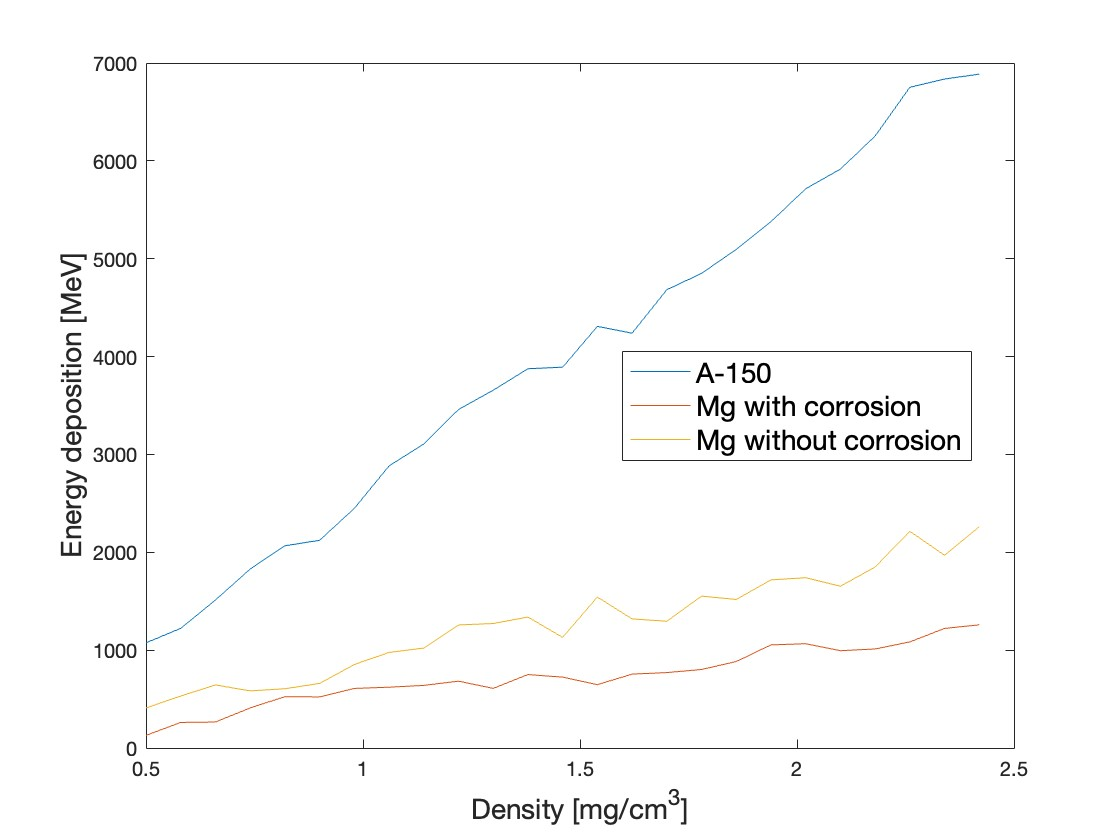
\includegraphics[scale = 0.32]{Master Thesis Manuel Galdon/figures/check source/energy deposition.jpg}
%    \caption{Energy deposition in the sensitive region of the PTW-33053 chamber with and without a hydromagnesite layer, and TE chamber.}
%  \label{fig:PTW-33053 with hydromagnesite. Energy. Electrons}
%\end{figure}

